\documentclass[a4paper]{article}
\usepackage{hyperref}
\usepackage[english]{babel}
\usepackage[utf8]{inputenc}
\usepackage{amsmath}
\usepackage{graphicx}
\usepackage[colorinlistoftodos]{todonotes}

\title{Visualization of Bitcoin Blockchain(Progress Report)}

\author{Zhiyi Xu and Ruolan Zeng}

\date{\today}

\begin{document}
\maketitle

\begin{abstract}
Blockchain and Bitcoin are both hot topics these days. Bitcoin is a distributed, decentralized crypto-currency. It uses the blockchain protocol to serialize transactions of the Bitcoin currency among its users. Below is an image briefly introducing how blockchain works for bitcoin. It’s a learning project and we want to mock and visualize Bitcoin blockchain. After that, we want to learn and try to implement Bitcoin-NG (Next Generation), a new blockchain protocol designed to scale, presented in Bitcoin-NG: A Scalable Blockchain Protocol. It is a Byzantine fault tolerant blockchain protocol that is robust to extreme churn and shares the same trust model as Bitcoin. Finally, we want to compare the transaction frequency, consensus latency, fairness, mining power utilization, time to win and time to prune of Bitcoin and Bitcoin-NG at the same block frequency or block size to see if Bitcoin-NG can reduce latency and increase throughput, and whether it is possible to improve the scalability of blockchain protocols to the point where the consensus latency is limited solely by the network diameter and the throughput bottleneck lies only in node processing power.

\end{abstract}

\section{First week: 10/25 - 10/31}
We found an implementation of blockchain in JavaScript(Figure 1):

\href{https://blockchaindemo.io}{https://blockchaindemo.io}

The reason we chose JavaScript as the language is that blockchain can be a very abstract concept and takes a relatively longer time for people to understand. In this case, the use of visualization can be very helpful. Using this implementation as a base, we plan to implement the Bitcoin-NG version on the top of it.

Right now, the implementation required users to create new blocks and setup for different peers. We plan to change it to a format that take in a database and automatically go through all the steps. It's in details but the data size is small, and it cannot offer users a board view of what transactions are happening behind the blockchain.
\begin{figure}
\centering
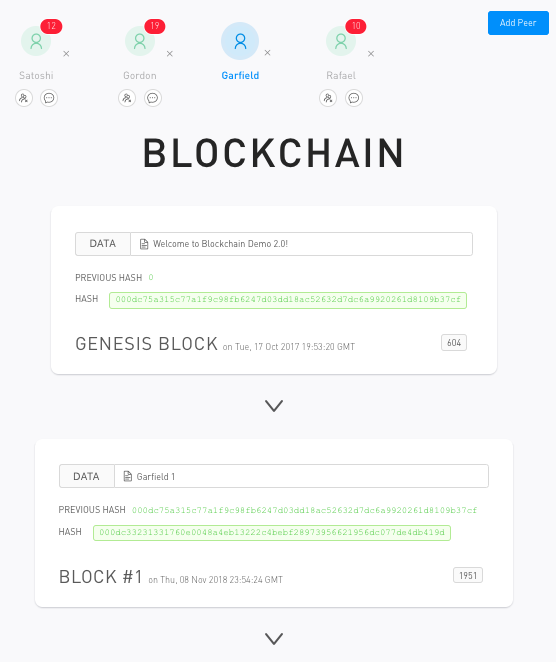
\includegraphics[width=1\textwidth]{blockchaindemo.png}
\caption{\label{fig:data}https://blockchaindemo.io}
\end{figure}

\section{Second week: 11/1 - 11/7}
We found another blockchain visualization(Figure 2):

\href{http://www.ethviewer.live}{http://www.ethviewer.live}

it’s a live application for Bitcoin that is implemented in Javascript. It’s nice visualization but the data size is big and the information is not in details. It offers users a board view of the transactions and blockchain, but give users little information inside each block. 
\begin{figure}
\centering
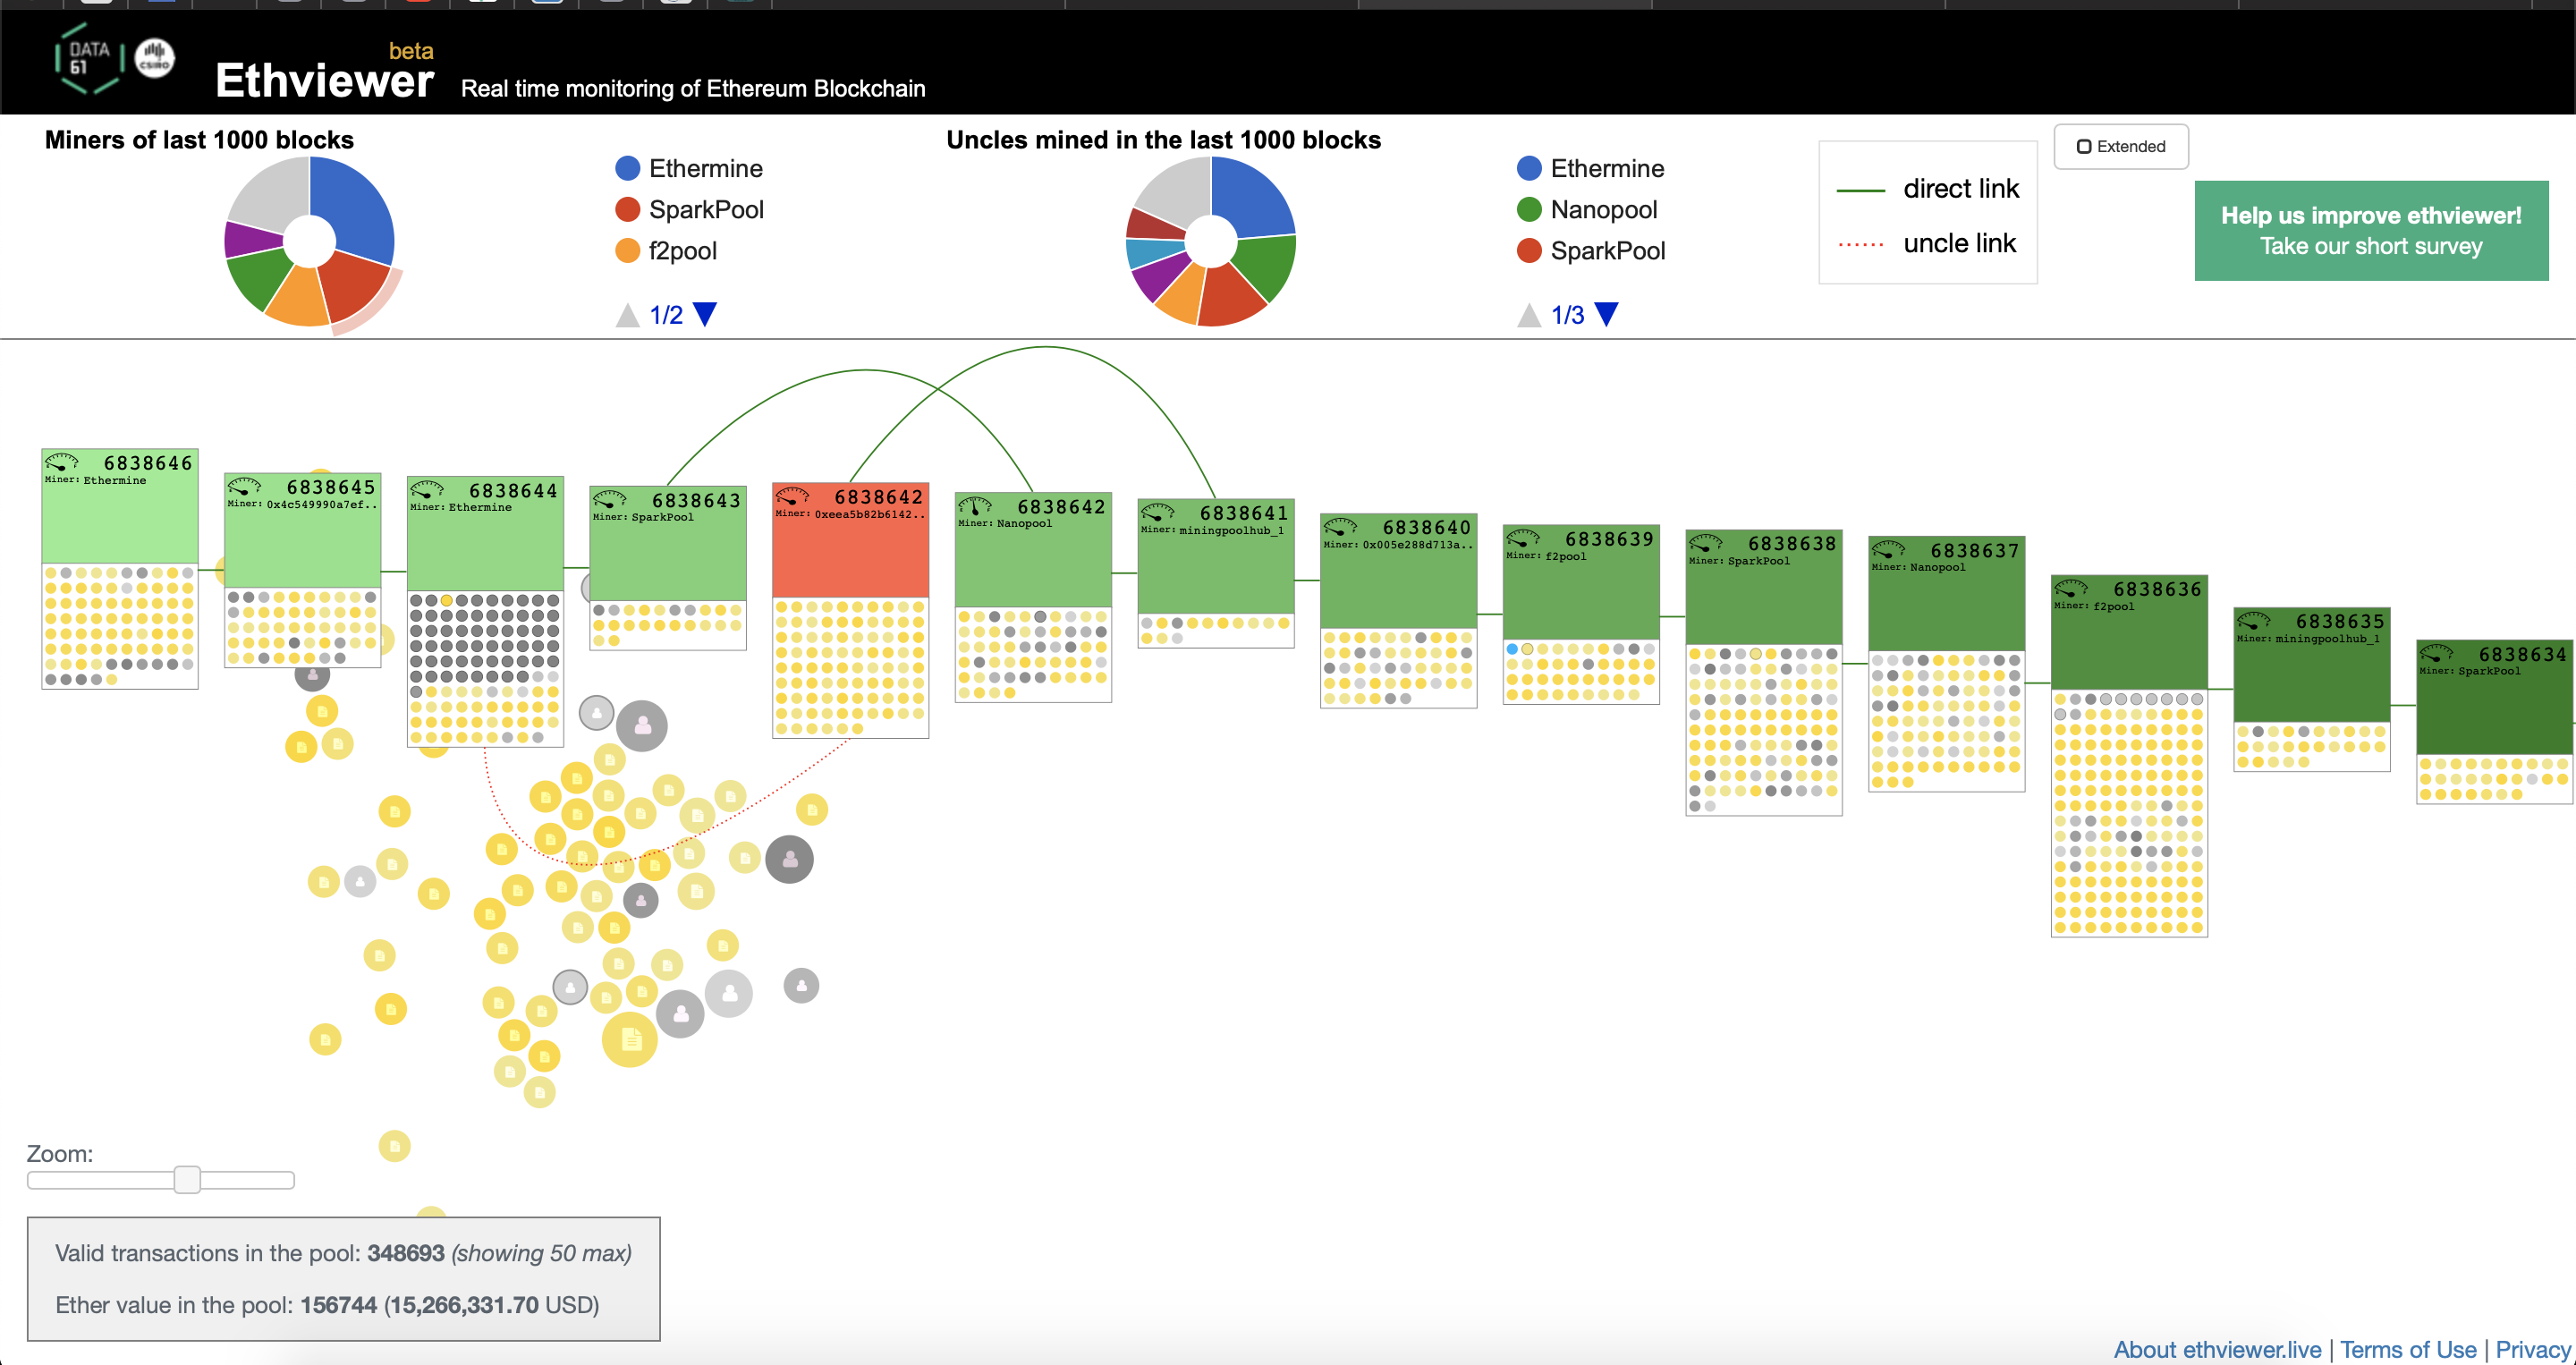
\includegraphics[width=1\textwidth]{liveblockchain.png}
\caption{\label{fig:data}http://www.ethviewer.live}
\end{figure}

\section{Third week: 11/8 - 11/29}
Due to the fire in California, our work is delayed. We decided to combine the advantages of both visualizations and made our first design for the visualization(Figure 3).

For the two graphs on the right side, we think despite Bitcoin’s potential, blockchain protocols face a significant scalability barrier. The maximum rate at which these systems can process transactions is capped by the choice of two parameters: block size and block interval:

	(1)Increasing block size improves throughput, but the resulting bigger blocks take longer to propagate in the network.
	
	(2)Reducing the block interval reduces latency, but leads to instability where the system is in disagreement and the blockchain is subject to reorganization.
	
So the graphs on the right side are the evaluation methodology. The main purpose of this learning project is to find out of the Bitcoin-NG concept can help to improve the efficiency of the blockchain. We plan to design a set of data and run the two different versions and compare the time that it took for they to go through everything.

We also get reference from \href{https://www.blockchain.com}{https://www.blockchain.com} and mock our users and transactions data(Figure 4).
\begin{figure}
\centering
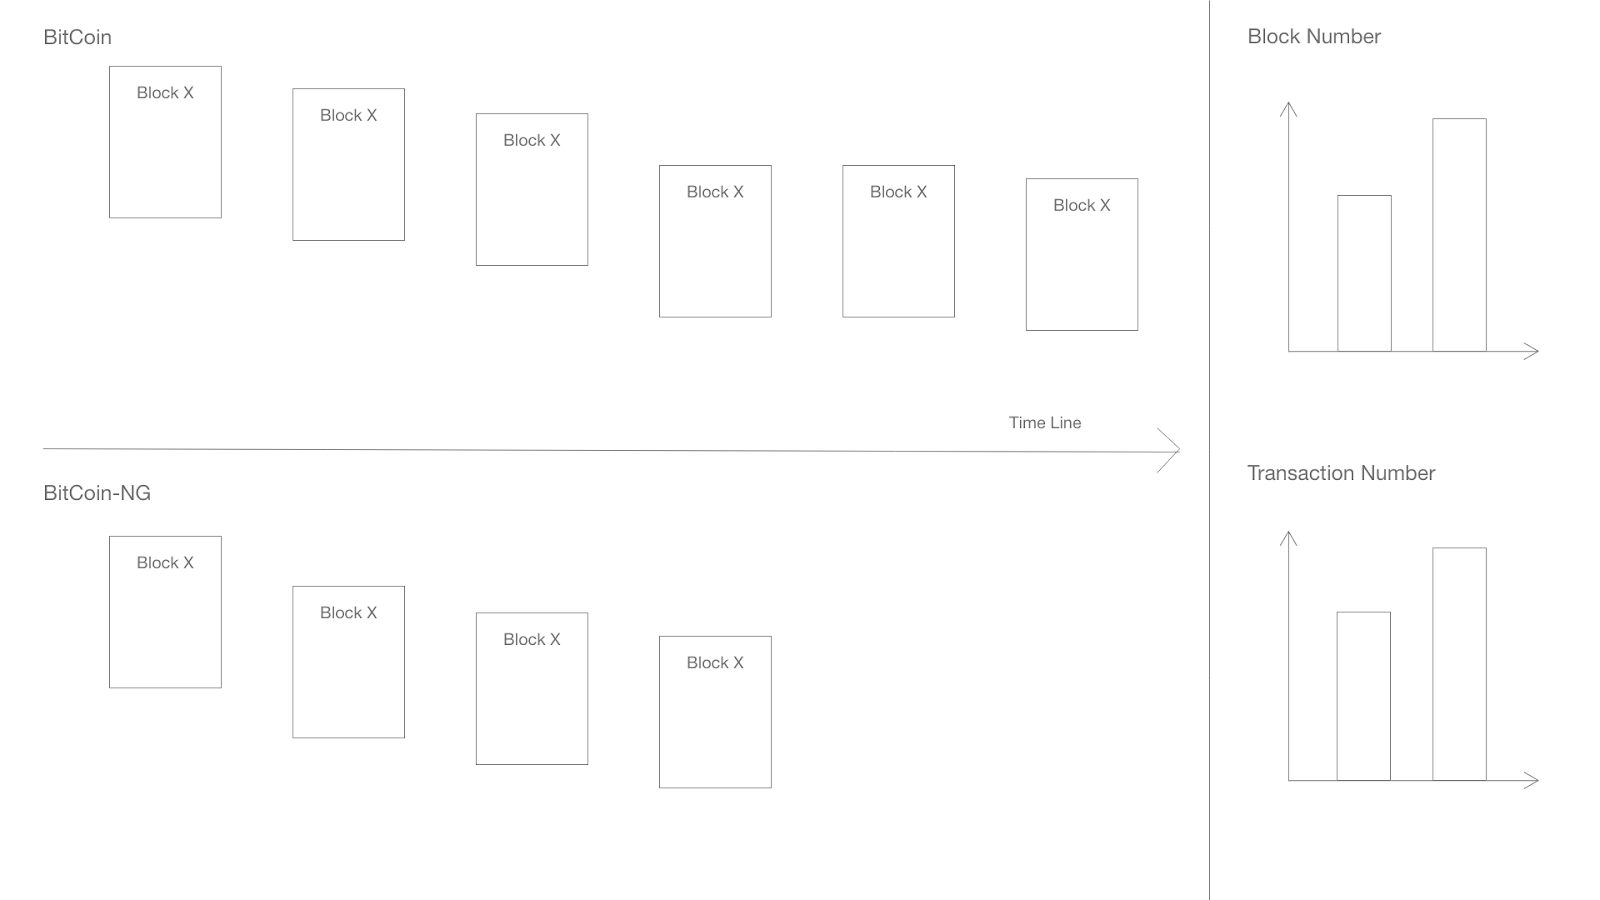
\includegraphics[width=1\textwidth]{firstdesign.png}
\caption{\label{fig:data}our first naive design for the visualization}
\end{figure}

\begin{figure}
\centering
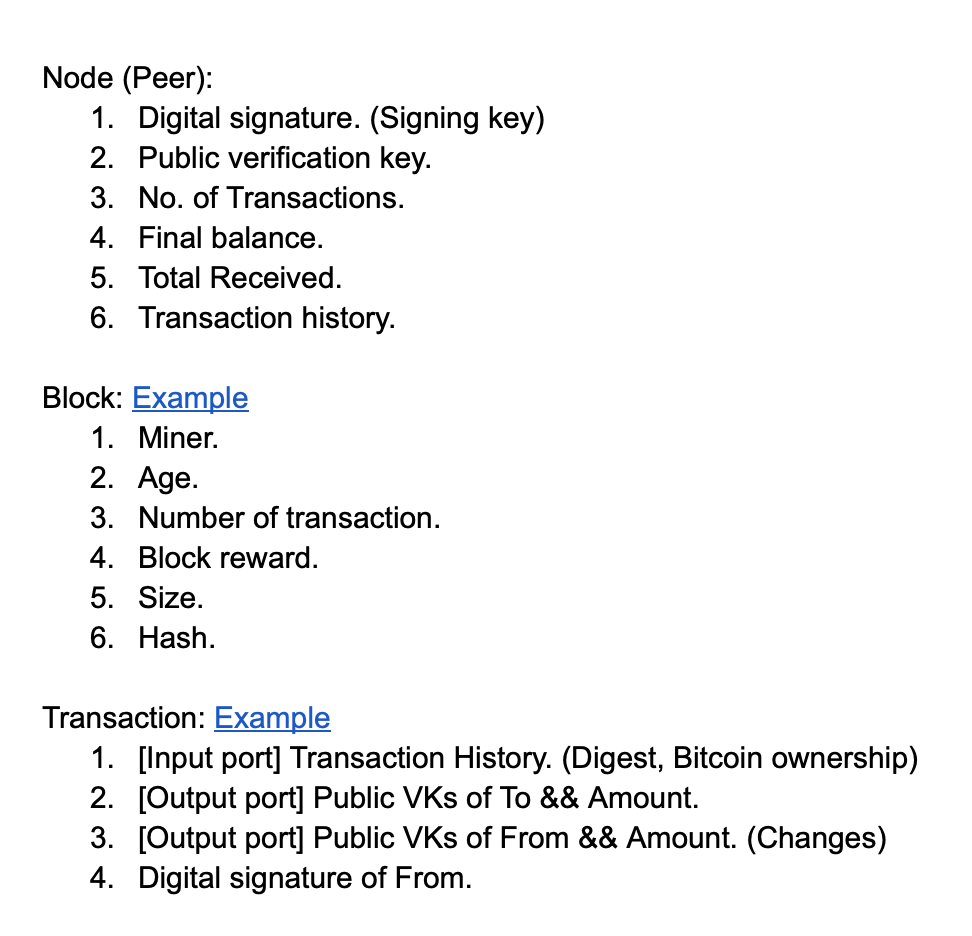
\includegraphics[width=1\textwidth]{datastructure.png}
\caption{\label{fig:data}structure of our data}
\end{figure}

\section{Fourth week: 11/30 - 12/6}
We finished a naive visualization for Bitcoin blockchain on web now(Figure 5), it still needs improvement. The link is

\href{https://github.com/LTZX/BitCoin-Visualization}{https://github.com/LTZX/BitCoin-Visualization}

\begin{figure}
\centering
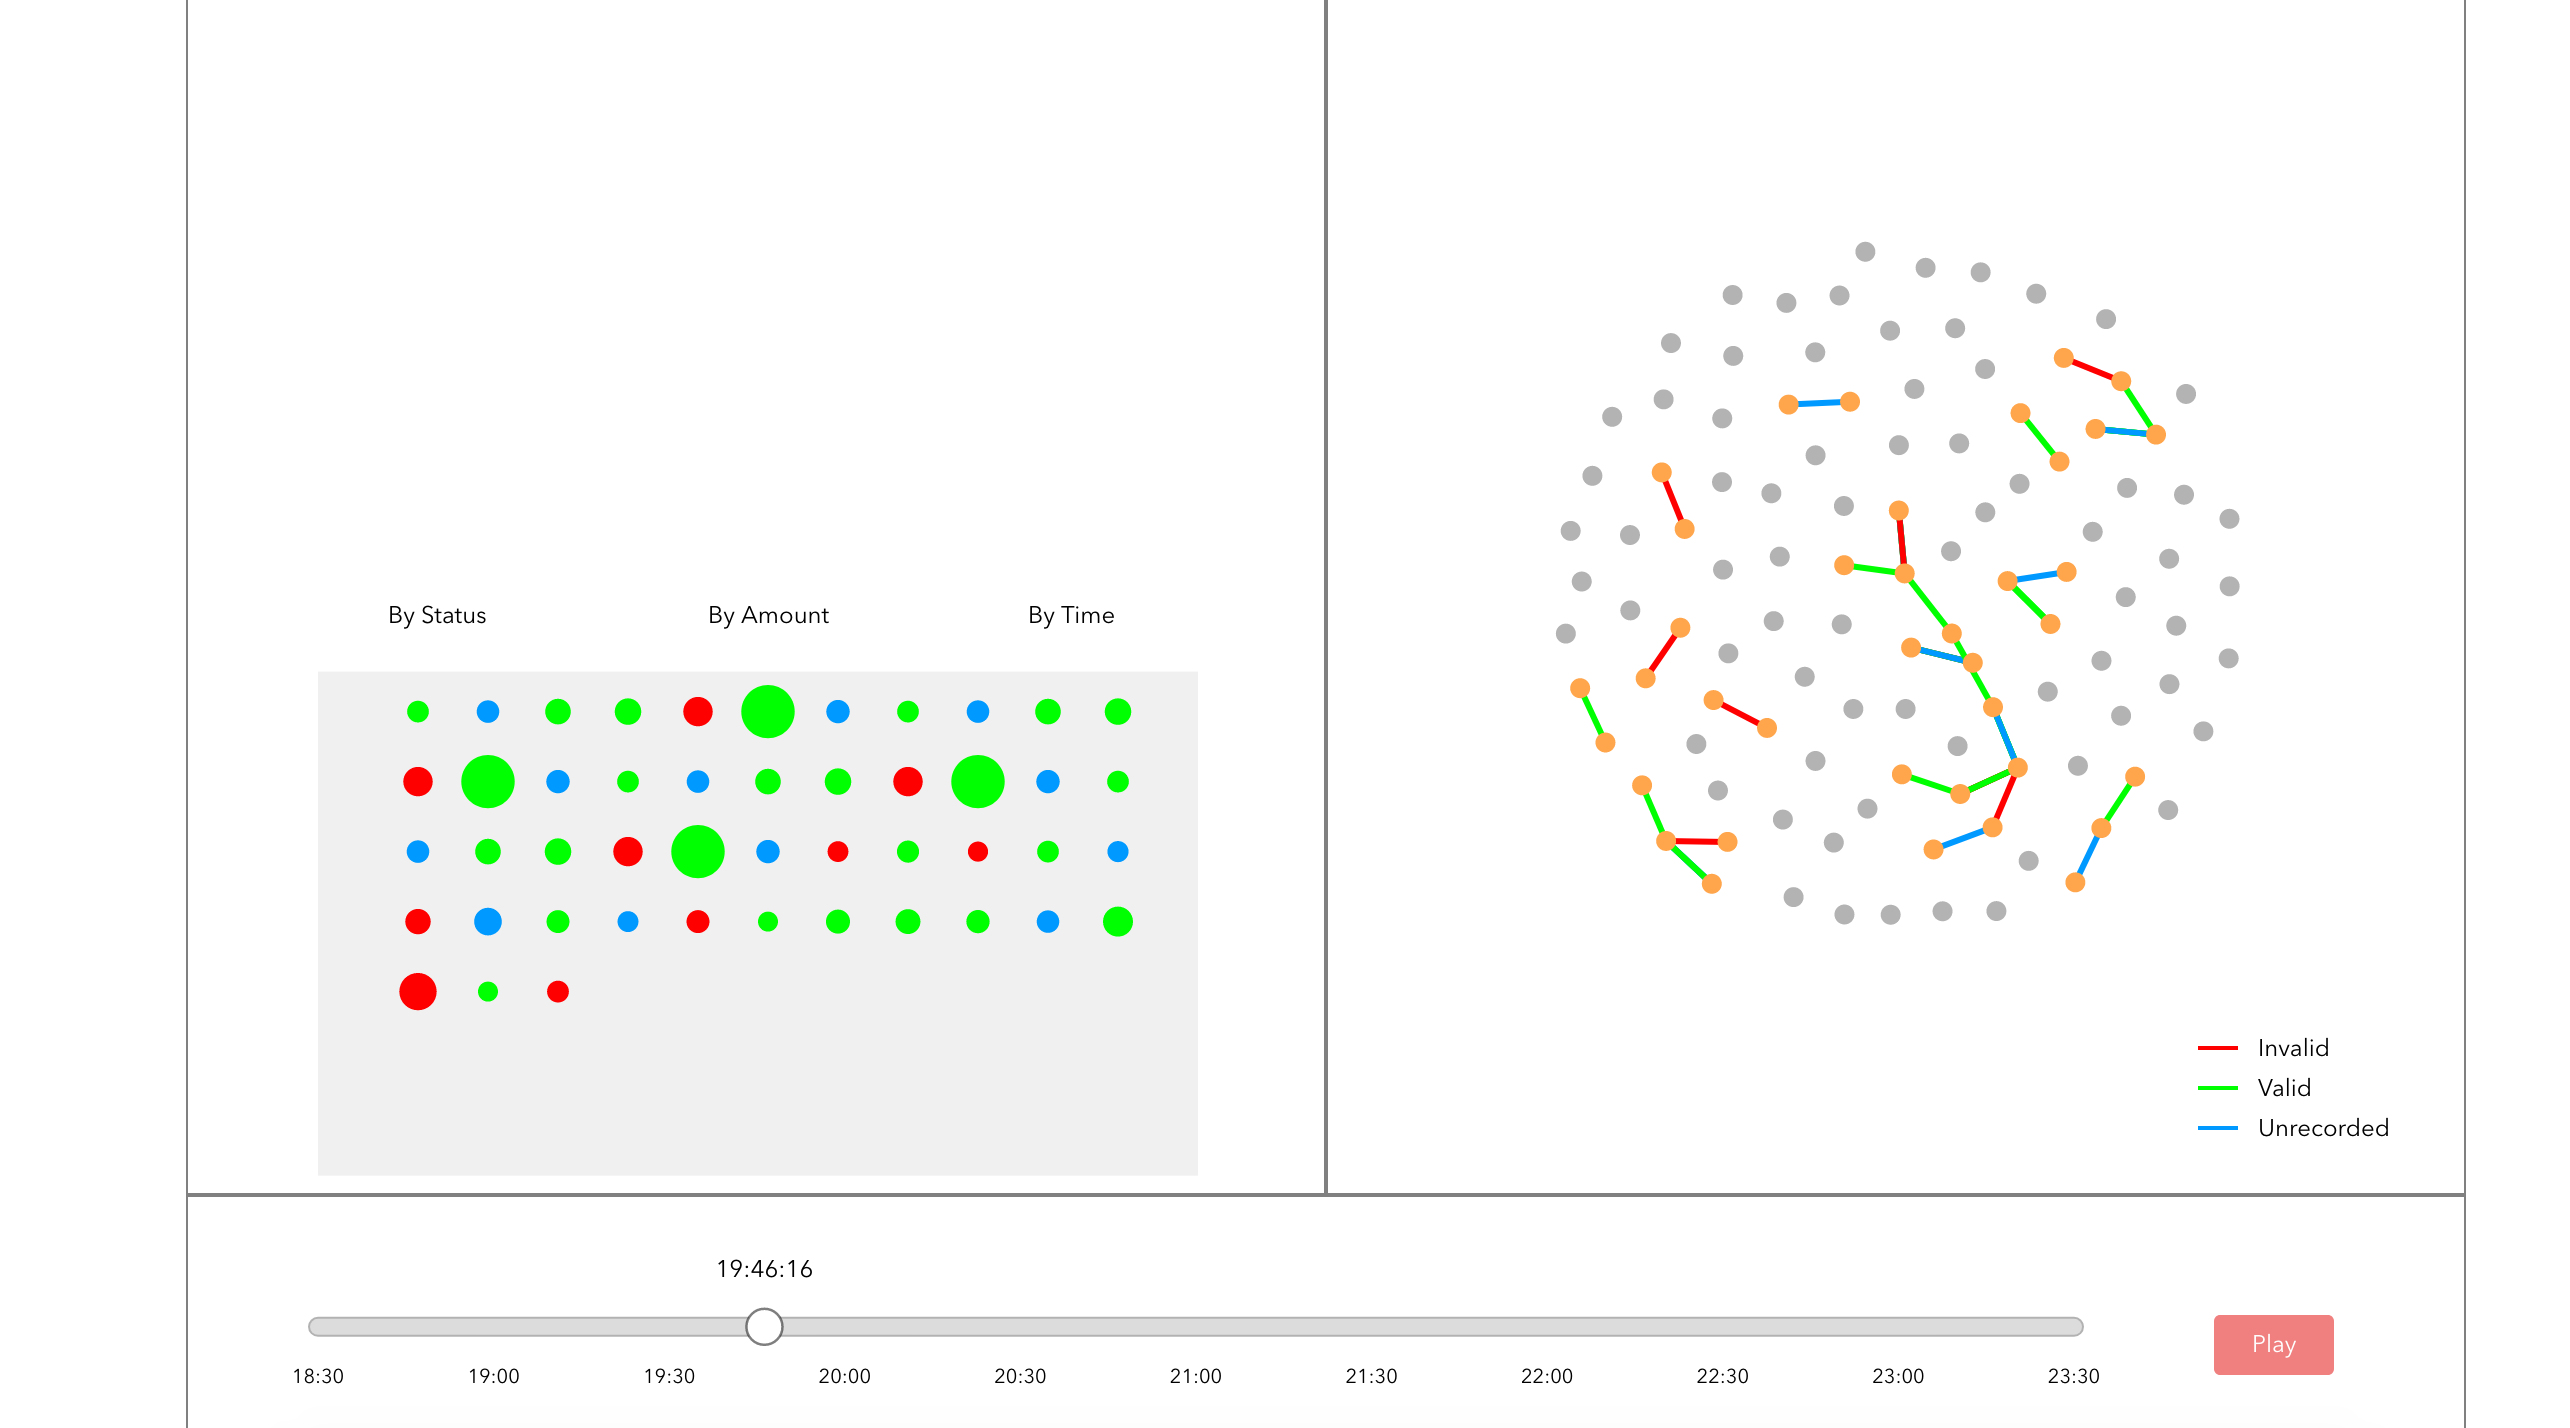
\includegraphics[width=1\textwidth]{visualization.png}
\caption{\label{fig:data}Our naive visualization on web}
\end{figure}

\section{Fiveth week: 12/7 - 12/16}
Our visualization is on this web and we are still updating it.

We'll add a visualization for the Bitcoin-NG as a comparison, and add the block number and transaction size graphs on the right side as addressed in our first design.

\end{document}